% !TEX program = pdflatex
% Statistical Physics Homework_1
\documentclass[12pt,a4paper]{article}
\usepackage[margin=1in]{geometry} 
\usepackage{amsmath,amsthm,amssymb,amsfonts,enumitem,fancyhdr,color,comment,graphicx,environ}
\pagestyle{fancy}
\setlength{\headheight}{65pt}
\newenvironment{problem}[2][Problem]{\begin{trivlist}
\item[\hskip \labelsep {\bfseries #1}\hskip \labelsep {\bfseries #2.}]}{\end{trivlist}}
\newenvironment{sol}
    {\emph{Solution:}
    }
    {
    \qed
    }
\specialcomment{com}{ \color{blue} \textbf{Comment:} }{\color{black}} %for instructor comments while grading
\NewEnviron{probscore}{\marginpar{ \color{blue} \tiny Problem Score: \BODY \color{black} }}
\usepackage[UTF8]{ctex}
\lhead{Name: 陈稼霖\\ StudentID: 45875852}
\rhead{PHYS1503 \\ Statistical Physics \\ Semester Fall 2019 \\ Assignment 1}
\begin{document}
\begin{problem}{1-2}
证明任何一种具有两个独立参量$T$, $p$的物质,其物态方程可由实验测得的体胀系数$\alpha$及等温压缩系数$\kappa_T$,根据下述积分求得
\[
\ln V=\int(\alpha dT-\kappa_Tdp)
\]

如果$\alpha=\frac{1}{T}$, $\kappa_T=\frac{1}{p}$,试求物态方程。
\end{problem}
\begin{sol}
\begin{gather}
V=V(p,T)
\Longrightarrow dV=\left(\frac{\partial V}{\partial T}\right)_pdT+\left(\frac{\partial V}{\partial p}\right)_Tdp
\end{gather}
代入体胀系数的定义
\begin{equation}
\alpha=\frac{1}{V}\left(\frac{\partial V}{\partial T}\right)_p
\end{equation}
和等温压缩系数的定义
\begin{equation}
\kappa_T=-\frac{1}{V}\left(\frac{\partial V}{\partial p}\right)_T
\end{equation}
得
\begin{gather}
dV=\alpha VdT-\kappa_TVdp\\
\Longrightarrow\frac{dV}{V}=\alpha dT-\kappa_Tdp
\end{gather}
两边同积分得
\begin{equation}
\ln V=\int(\alpha dT-\kappa_Tdp)
\end{equation}
代入$\alpha=\frac{1}{T}$, $\kappa_T=\frac{1}{p}$得
\begin{gather}
\ln V=\ln T-\ln p+C_1\\
\Longrightarrow\frac{pV}{T}=C
\end{gather}
其中$C$为一常数。
\end{sol}

\begin{problem}{1-5}
描述金属丝的几何参量是长度$L$,力学参量是张力$\mathcal{T}$,物态方程是
\[
f(\mathcal{T},L,T)=0
\]
实验通常在$1p_n$下进行,其体积变化可以忽略。

线膨胀系数定义为
\[
\alpha=\frac{1}{L}\left(\frac{\partial L}{\partial T}\right)_{\mathcal{T}}
\]
等温杨氏模量定义为
\[
Y=\frac{L}{A}\left(\frac{\partial\mathcal{T}}{\partial L}\right)_T
\]
其中$A$是金属丝的截面积。一般来说,$\alpha$和$Y$是$T$的函数,对于$\mathcal{T}$仅有微弱的依赖关系。如果温度变化范围不大,可以看做常量。假设金属丝两端固定。试证明,当温度由$T_1$降至$T_2$时,其张量的增加为
\[
\Delta\mathcal{T}=-YA\alpha(T_2-T_1)
\]
\end{problem}
\begin{sol}
根据循环关系和互逆关系
\begin{gather}
\left(\frac{\partial\mathcal{T}}{\partial T}\right)_L\left(\frac{\partial T}{\partial L}\right)_{\mathcal{T}}\left(\frac{\partial L}{\partial \mathcal{T}}\right)_{T}=-1,\quad\left(\frac{\partial T}{\partial L}\right)_{\mathcal{T}}\left(\frac{\partial L}{\partial T}\right)_{\mathcal{T}}\left(\frac{\mathcal{T}}{\mathcal{L}}\right)_T=1,\quad\left(\frac{\partial L}{\partial\mathcal{T}}\right)_T\left(\frac{\partial\mathcal{T}}{\partial L}\right)_T=1\\
\Longrightarrow\left(\frac{\partial\mathcal{T}}{\partial T}\right)_L=-\left(\frac{\partial L}{\partial T}\right)_{\mathcal{T}}\left(\frac{\partial\mathcal{T}}{\partial L}\right)_T
\end{gather}
代入线性膨胀系数和等温杨氏模量的定义得
\begin{equation}
\left(\frac{\partial\mathcal{T}}{\partial T}\right)_L=-YA\alpha
\end{equation}
两边同对$T$积分得
\begin{equation}
\Delta\mathcal{T}=-YA\alpha(T_2-T_1)
\end{equation}
\end{sol}

\begin{problem}{1-9}
试证明:理想气体在某一过程中的热容量$C_n$如果是常量,该过程一定是多方过程,多方指数$n=\frac{C_n-C_p}{C_n-C_V}$。

即设气体的定压热容量和定容热容量是常数。
\end{problem}
\begin{sol}
热容量定义
\begin{equation}
C_n=\lim_{\Delta T\rightarrow0}\frac{\Delta Q}{\Delta T}
\end{equation}
根据热力学第一定律
\begin{gather}
C_n=\frac{dU+pdV}{dT}=\frac{C_VdT+pdV}{dT}\\
\label{Cn}(C_n-C_V)dT=pdV
\end{gather}
对理想气体状态方程
\begin{equation}
pV=nRT
\end{equation}
微分得
\begin{equation}
Vdp+pdV=nRdT
\end{equation}
代入式(\ref{Cn})中得
\begin{gather}
\frac{C_n-C_V}{nR}(Vdp+pdV)=pdV\\
\Longrightarrow(C_n-C_V)\frac{dp}{p}=-(C_n-C_V-nR)\frac{dV}{V}\\
\Longrightarrow(C_n-C_V)\frac{dp}{p}=-(C_n-C_p)\frac{dV}{V}
\end{gather}
两边积分得
\begin{equation}
pV^{\frac{C_n-C_p}{C_n-C_V}}=C
\end{equation}
故该过程一定是多方过程,多方指数$n=\frac{C_n-C_p}{C_n-C_V}$。
\end{sol}

\begin{problem}{1-11}
大气温度随高度降低的重要原因是在对流层中不同高度之间的空气不断发生对流。由于气压随高度而降低,空气上升时膨胀,下降时收缩。空气的导热率很小,膨胀和收缩的过程可以认为是绝热过程。试计算大气温度随高度的变化率,并给出数值结果。
\end{problem}
\begin{sol}
流体压强公式
\begin{gather}
dp=-\rho gdz\\
\frac{dp}{dz}=-\rho g
\end{gather}
绝热过程中空气压强与温度的关系
\begin{gather}
\frac{p^{\gamma-1}}{T^{\gamma}}=C\\
\Longrightarrow T=C^{-1/\gamma}p^{(\gamma-1)/\gamma}
\end{gather}
其中$C$为一常数,两边同取微分
\begin{gather}
dT=\frac{\gamma-1}{\gamma}\frac{C^{-1/\gamma}p^{(\gamma-1)/\gamma}}{p}dp\\
\Longrightarrow\frac{dT}{dp}=\frac{\gamma-1}{\gamma}\frac{T}{p}
\end{gather}
代入理想气体状态方程得
\begin{gather}
\frac{dT}{dp}=\frac{\gamma-1}{\gamma}\frac{V}{nR}=\frac{\gamma-1}{\gamma}\frac{m^+}{\rho R}
\end{gather}
其中$m^+$为空气的摩尔质量。\\
根据链式法则,大气温度随高度的变化关系
\begin{equation}
\frac{dT}{dz}=\frac{dT}{dp}\frac{dp}{dz}=-\frac{\gamma-1}{\gamma}\frac{m^+}{\rho R}\rho g=-\frac{\gamma-1}{\gamma}\frac{m^+g}{R}
\end{equation}
代入空气的比热容比$\gamma=1.40$,空气的摩尔质量$m^+=29\times10^{-3}\text{kg}\cdot\text{mol}^{-1}$,摩尔气体常量$R=8.3145\text{J}\cdot\text{mol}^{-1}\cdot\text{K}^{-1}$,重力加速度$g=9.8\text{m}\cdot\text{s}^{-2}$得大气温度随高度的变化率为
\begin{equation}
\frac{dT}{dz}=9.8\times10^{-3}\text{K}\cdot\text{m}^{-1}=9.8\text{K}\cdot\text{km}^{-1}
\end{equation}
\end{sol}

\begin{problem}{1-14}
试根据热力学第二定律证明两条绝热线不能相交。
\end{problem}
\begin{sol}
反证法:假设两条绝热线相交,交点为$C$,则必然可以找到一条等温线,与两条绝热线均相交,交点分别为$A$和$B$,如图\ref{Homework_1_1_14}。对于循环$A\rightarrow B\rightarrow C\rightarrow A$,系统在过程$A\rightarrow B$中从外界吸收热量,整个循环对外做正功。这违背了热力学第二定律的描述 -- 不可能从单一热源吸热使之完全变成有用的功而不引起其他变化,因此假设错误,两条绝热线不能相交。
\begin{figure}[h]
\centering
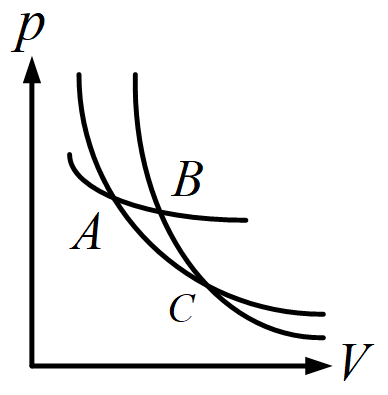
\includegraphics[scale=0.5]{Homework_1_1-14.png}
\caption{1-14题图} \label{Homework_1_1_14}
\end{figure}
\end{sol}

\begin{problem}{1-16}
理想气体分别经过等压过程和等容过程,温度由$T_1$升至$T_2$。假设$\gamma$是常数,试证明前者的熵增为后者的$\gamma$倍。
\end{problem}
\begin{sol}
等压过程熵增
\begin{equation}
\Delta S_p=\int_{T_1}^{T_2}\frac{dQ}{T}=\int_{T_1}^{T_2}\frac{C_pdT}{T}=C_p\ln\frac{T_2}{T_1}
\end{equation}
等容过程熵增
\begin{equation}
\Delta S_V=\int_{T_1}^{T_2}\frac{dQ}{T}=\int_{T_1}^{T_2}\frac{C_VdT}{T}=C_V\ln\frac{T_2}{T_1}
\end{equation}
前后两者之比为
\begin{equation}
\frac{\Delta S_p}{\Delta S_V}=\frac{C_p}{C_V}=\gamma
\end{equation}
\end{sol}

\begin{problem}{1-17}
温度为$0^{\circ}$C的$1$kg水与温度为$100^{\circ}$C的恒温热源接触后,水温达到$100^{\circ}$C。试分别求水和热源的熵变以及整个系统的总熵变。欲使整个系统的熵保持不变,应如何使水温从$0^{\circ}$升至$100^{\circ}$C?已知水的比热容为$4.18\text{J}\cdot\text{g}^{-1}\cdot\text{K}^{-1}$。
\end{problem}
\begin{sol}
水的熵变
\begin{equation}
\Delta S_{\text{water}}=\int_{273.15}^{373.15}\frac{dQ}{T}=\int_{273.15}^{373.15}\frac{m_{\text{water}}C_{\text{water}}dT}{T}=m_{\text{water}}C_{\text{water}}\ln\frac{373.15}{273.15}=1304\text{J}\cdot\text{K}^{-1}
\end{equation}
水从热源吸收的热量
\begin{equation}
\Delta Q=m_{\text{water}}C_{\text{water}}(373.15-273.15)=4.18\times10^5\text{J}
\end{equation}
热源的熵变
\begin{equation}
\Delta S_{\text{heat source}}=\frac{-\Delta Q}{373.15}=-1120\text{J}\cdot\text{K}^{-1}
\end{equation}
整个系统的总熵变
\begin{equation}
\Delta S_{\text{system}}=\Delta S_{\text{water}}+\Delta S_{\text{heat source}}=184\text{J}\cdot\text{K}^{-1}
\end{equation}
欲使整个系统的熵保持不变,应使水与一系列温度分布在从$0^{\circ}$C到$100^{\circ}$C的热源依次接触,通过可逆的吸热过程,使水温从$0^{\circ}$C缓慢地上升到$100^{\circ}$C。
\end{sol}

\begin{problem}{1-19}
均匀杆的温度一端为$T_1$,另一端为$T_2$。试计算达到均匀温度$\frac{1}{2}(T_2-T_1)$后的熵增。
\end{problem}
\begin{sol}
均匀杆达到均匀温度的熵增为
\begin{align}
\nonumber\Delta S=&\int_0^Ldl\int_{T_1+\frac{T_2-T_1}{L}l}^{\frac{T_1+T_2}{2}}\frac{\frac{C_p}{m}\rho dldT}{T}\\
\nonumber=&\frac{C_p}{m}\rho\int_0^Ldl\ln\frac{\frac{T_1+T_2}{2}}{T_1+\frac{T_2-T_1}{L}l}\\
\nonumber=&\frac{C_p}{m}\rho L\left(\ln\frac{T_1+T_2}{2}-\frac{T_2\ln T_2-T_1\ln T_1}{T_2-T_1}+1\right)\\
=&C_p\left(\ln\frac{T_1+T_2}{2}-\frac{T_2\ln T_2-T_1\ln T_1}{T_2-T_1}+1\right)
\end{align}
\end{sol}
\end{document}